%%%---PREAMBLE---%%%%%%%%%%%%%%%%%%%%%%%%%%%%
\documentclass[twoside,12pt,final]{ucthesis-CA2012}

% fix for pandoc 1.14
\providecommand{\tightlist}{%
  \setlength{\itemsep}{0pt}\setlength{\parskip}{0pt}}

%--- Packages ---------------------------------------------------------
\usepackage[lofdepth,lotdepth,caption=false]{subfig}
\usepackage{fancyhdr}
\usepackage{amsmath, amssymb, graphicx}
\usepackage{xspace}
\usepackage{braket}
\usepackage{color}
\usepackage{setspace}
\usepackage{fancyvrb}
\usepackage{array}
\usepackage{ifxetex,ifluatex}
\usepackage{etoolbox}

%% for the per mil symbol
\usepackage[nointegrals]{wasysym}

% more attractive tables
\usepackage{booktabs}
\usepackage{xcolor}
\usepackage{tabu}
\usepackage{tabularx}
\usepackage{lscape}
\usepackage{longtable}
\usepackage{titlesec}


\usepackage[nostamp]{draftwatermark}
% % Use the following to make modification
\SetWatermarkText{DRAFT}
\SetWatermarkLightness{0.95}

%---New Definitions and Commands------------------------------------------------------

\newtheorem{theorem}{Jibberish}

\bibliography{references}

\hyphenation{mar-gin-al-ia}

% from uw_template.tex

% commands and environments needed by pandoc snippets
% extracted from the output of `pandoc -s`
%% Make R markdown code chunks work

\ifxetex
  \usepackage{fontspec,xltxtra,xunicode}
  \defaultfontfeatures{Mapping=tex-text,Scale=MatchLowercase}
\else
  \ifluatex
    \usepackage{fontspec}
    \defaultfontfeatures{Mapping=tex-text,Scale=MatchLowercase}
  \else
    \usepackage[utf8]{inputenc}
  \fi
\fi
\DefineShortVerb[commandchars=\\\{\}]{\|}
\DefineVerbatimEnvironment{Highlighting}{Verbatim}{commandchars=\\\{\}}
% Add ',fontsize=\small' for more characters per line
\newenvironment{Shaded}{}{}
\newcommand{\KeywordTok}[1]{\textcolor[rgb]{0.00,0.44,0.13}{\textbf{{#1}}}}
\newcommand{\DataTypeTok}[1]{\textcolor[rgb]{0.56,0.13,0.00}{{#1}}}
\newcommand{\DecValTok}[1]{\textcolor[rgb]{0.25,0.63,0.44}{{#1}}}
\newcommand{\BaseNTok}[1]{\textcolor[rgb]{0.25,0.63,0.44}{{#1}}}
\newcommand{\FloatTok}[1]{\textcolor[rgb]{0.25,0.63,0.44}{{#1}}}
\newcommand{\CharTok}[1]{\textcolor[rgb]{0.25,0.44,0.63}{{#1}}}
% Added lines below after bug and recommendation : https://tex.stackexchange.com/questions/660787/undefined-control-sequence-for-normaltok-or-specialchartok

\newcommand{\ConstantTok}[1]{\textcolor[rgb]{0.53,0.00,0.00}{{#1}}}
\newcommand{\SpecialCharTok}[1]{\textcolor[rgb]{0.25,0.44,0.63}{{#1}}}
\newcommand{\AttributeTok}[1]{\textcolor[rgb]{0.49,0.56,0.16}{{#1}}}
\newcommand{\StringTok}[1]{\textcolor[rgb]{0.25,0.44,0.63}{{#1}}}
\newcommand{\CommentTok}[1]{\textcolor[rgb]{0.38,0.63,0.69}{\textit{{#1}}}}
\newcommand{\OtherTok}[1]{\textcolor[rgb]{0.00,0.44,0.13}{{#1}}}
\newcommand{\AlertTok}[1]{\textcolor[rgb]{1.00,0.00,0.00}{\textbf{{#1}}}}
\newcommand{\FunctionTok}[1]{\textcolor[rgb]{0.02,0.16,0.49}{{#1}}}
\newcommand{\RegionMarkerTok}[1]{{#1}}
\newcommand{\ErrorTok}[1]{\textcolor[rgb]{1.00,0.00,0.00}{\textbf{{#1}}}}
\newcommand{\NormalTok}[1]{{#1}}
\newcommand{\OperatorTok}[1]{\textcolor[rgb]{0.00,0.44,0.13}{\textbf{{#1}}}}
\newcommand{\BuiltInTok}[1]{\textcolor[rgb]{0.00,0.44,0.13}{\textbf{{#1}}}}
\newcommand{\ControlFlowTok}[1]{\textcolor[rgb]{0.00,0.44,0.13}{\textbf{{#1}}}}

\ifxetex
  \usepackage[setpagesize=false, % page size defined by xetex
              unicode=false, % unicode breaks when used with xetex
              xetex,
              colorlinks=true,
              linkcolor=blue]{hyperref}
\else
  \usepackage[unicode=true,
              colorlinks=true,
              linkcolor=blue]{hyperref}
\fi
\hypersetup{breaklinks=true, pdfborder={0 0 0}}
\setlength{\parindent}{0pt}
\setlength{\parskip}{6pt plus 2pt minus 1pt}
\setlength{\emergencystretch}{3em}  % prevent overfull lines
\setcounter{secnumdepth}{0}

%---Set Margins ------------------------------------------------------
\setlength\oddsidemargin{0.25 in} \setlength\evensidemargin{0.25 in} \setlength\textwidth{6.25 in} \setlength\textheight{8.50 in}
\setlength\footskip{0.25 in} \setlength\topmargin{0 in} \setlength\headheight{0.25 in} \setlength\headsep{0.25 in}

%%%---DOCUMENT---%%%%%%%%%%%%%%%%%%%%%%%%%%%%
\begin{document}

%=== Preliminary Pages ============================================
\begin{ucfrontmatter}

  %%%%%%%%%%%%%%%%%%%%%%%%%%%
  % TITLE PAGE INFORMATION %  modified to meet UCDavis, R. Peek, 2018
  %%%%%%%%%%%%%%%%%%%%%%%%%%%

  \title{Organic Seed Systems}
  \author{Liza Wood}

\report{DISSERTATION} 
  \degree{DOCTOR OF PHILOSOPHY} 
  \degreemonth{September} \degreeyear{2023}
  \chair{Mark Lubell}  % this is your advisor
  \othermemberA{Tyler Scott} % This is a member of your committee
  \othermemberB{Neil McRoberts} % This is a member of your committee
  \othermemberC{} % This is a member of your committee
  \numberofmembers{3} % should match the number of entries above (chair + othermembers)
  \field{ECOLOGY}
  \campus{DAVIS}
  
	\maketitle
	
	% APPROVAL AND COPYRIGHT
	% \approvalpage % AS OF 2018 Fall, don't need this additional page if use cover page for signatures
	\copyrightpage

  %%%%%%%%%%%%%%%%%%%%%%%%%%%
  % DEDICATION PAGE INFORMATION %
  %%%%%%%%%%%%%%%%%%%%%%%%%%%
    \begin{dedication}

      \vspace*{20ex}
      \begin{center}
      \begin{large}

        

      \end{large}
      \end{center}
  \end{dedication}
  % ACKNOWLEDGEMENTS
\begin{acknowledgements}
    ``My acknowledgments''
  \end{acknowledgements}
  %%%%%%
  % CV % Not required, add if you need
  %%%%%%
%   \begin{vitae}
%     \addcontentsline{toc}{chapter}{Curriculum Vitae}
% 
%     \begin{vitaesection}{Education}
%     \vspace{-0.1cm}
%     \item [2018]	Ph.D. in Environmental Science and Management (Expected), University of California, Santa Barbara.
%     \item [2010]	MESM in in Environmental Science and Management, University of California, Santa Barbara.
%     \item [2007]	B.S. in Ecosystem Science and Policy and Biology, University of Miami
%     \end{vitaesection}
% 
%     \textbf{Publications}
% 
%     Anderson, S.C., Cooper, A.B., Jensen, O.P., Minto, C., Thorson, J.T., Walsh, J.C., Afflerbach, J., Dickey‐Collas, M., Kleisner, K.M., Longo, C., Osio, G.C., Ovando, D., Mosqueira, I., Rosenberg, A.A., Selig, E.R., n.d. Improving estimates of population status and trend with superensemble models. Fish and Fisheries 18, 732–741. https://doi.org/10.1111/faf.12200
% 
%  Burgess, M.G., McDermott, G.R., Owashi, B., Reeves, L.E.P., Clavelle, T., Ovando, D., Wallace, B.P., Lewison, R.L., Gaines, S.D., Costello, C., 2018. Protecting marine mammals, turtles, and birds by rebuilding global fisheries. Science 359, 1255–1258. https://doi.org/10.1126/science.aao4248
% 
% Costello, C., Ovando, D., Clavelle, T., Strauss, C.K., Hilborn, R., Melnychuk, M.C., Branch, T.A., Gaines, S.D., Szuwalski, C.S., Cabral, R.B., Rader, D.N., Leland, A., 2016. Global fishery prospects under contrasting management regimes. PNAS 113, 5125–5129. https://doi.org/10.1073/pnas.1520420113
% 
% \end{vitae}

	%%%%%%%%%%%%%%%%%%%%%%%%%%%
  % ABSTRACT %
  %%%%%%%%%%%%%%%%%%%%%%%%%%%
  \begin{abstract}
    \addcontentsline{toc}{chapter}{Abstract}

    ``Overall abstract?''

    %\abstractsignature
  \end{abstract}
  % TABLE OF CONTENTS
	\tableofcontents

	  \listoftables
  
    \listoffigures
  
\end{ucfrontmatter}
\begin{ucmainmatter}

\hypertarget{introduction}{%
\chapter*{Introduction}\label{introduction}}
\addcontentsline{toc}{chapter}{Introduction}

Short tying it all together

\hypertarget{ch1-adoption}{%
\chapter{Adoption of organic seed}\label{ch1-adoption}}

\chaptermark{adoption}
\begin{Shaded}
\begin{Highlighting}[]
\CommentTok{\# List of packages required for this analysis}
\NormalTok{pkg }\OtherTok{\textless{}{-}} \FunctionTok{c}\NormalTok{(}\StringTok{"dplyr"}\NormalTok{, }\StringTok{"ggplot2"}\NormalTok{, }\StringTok{"knitr"}\NormalTok{, }\StringTok{"bookdown"}\NormalTok{, }\StringTok{"devtools"}\NormalTok{)}
\FunctionTok{library}\NormalTok{(dplyr)}
\FunctionTok{library}\NormalTok{(ggplot2)}
\FunctionTok{library}\NormalTok{(kableExtra)}
\end{Highlighting}
\end{Shaded}
\hypertarget{introduction-1}{%
\section{Introduction}\label{introduction-1}}

\hypertarget{background}{%
\section{Background}\label{background}}

\hypertarget{empirical-approach}{%
\section{Empirical approach}\label{empirical-approach}}

\hypertarget{results}{%
\section{Results}\label{results}}
\begin{Shaded}
\begin{Highlighting}[]
\FunctionTok{library}\NormalTok{(knitr)}
\FunctionTok{kable}\NormalTok{(}\FunctionTok{head}\NormalTok{(cars),}
      \AttributeTok{longtable =} \ConstantTok{TRUE}\NormalTok{,}
      \AttributeTok{booktabs =} \ConstantTok{TRUE}\NormalTok{, }\AttributeTok{cap =} \StringTok{"Cars"}\NormalTok{) }\SpecialCharTok{\%\textgreater{}\%} \FunctionTok{kable\_styling}\NormalTok{()}
\end{Highlighting}
\end{Shaded}
\begin{longtable}[t]{rr}
\caption{\label{tab:maxdelays}Cars}\\
\toprule
speed & dist\\
\midrule
4 & 2\\
4 & 10\\
7 & 4\\
7 & 22\\
8 & 16\\
\addlinespace
9 & 10\\
\bottomrule
\end{longtable}
The last two options make the table a little easier-to-read.

We can further look into the properties of the largest value here for American Airlines Inc.~To do so, we can isolate the row corresponding to the arrival delay of 1539 minutes for American in our original \texttt{flights} dataset.

We see that the flight occurred on March 3rd and departed a little after 2 PM on its way to Dallas/Fort Worth. Lastly, we show how we can visualize the arrival delay of all departing flights from Portland on March 3rd against time of departure.
\begin{figure}
\centering
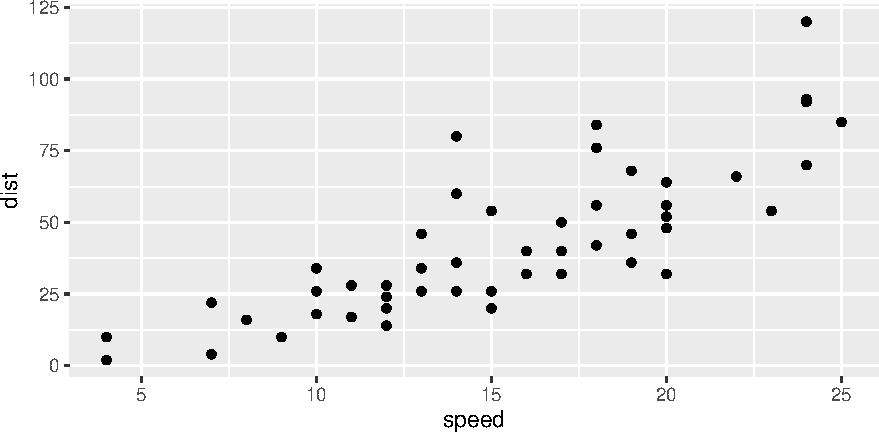
\includegraphics{thesis_files/figure-latex/march3plot-1.pdf}
\caption{\label{fig:march3plot}Cars}
\end{figure}
\hypertarget{discussion}{%
\section{Discussion}\label{discussion}}

\hypertarget{conclusion}{%
\section{Conclusion}\label{conclusion}}

\hypertarget{spatial}{%
\chapter{Spatial}\label{spatial}}

\chaptermark{spatial}
\begin{Shaded}
\begin{Highlighting}[]
\CommentTok{\# List of packages required for this analysis}
\NormalTok{pkg }\OtherTok{\textless{}{-}} \FunctionTok{c}\NormalTok{(}\StringTok{"dplyr"}\NormalTok{, }\StringTok{"ggplot2"}\NormalTok{, }\StringTok{"knitr"}\NormalTok{, }\StringTok{"bookdown"}\NormalTok{, }\StringTok{"devtools"}\NormalTok{)}
\FunctionTok{library}\NormalTok{(dplyr)}
\FunctionTok{library}\NormalTok{(ggplot2)}
\FunctionTok{library}\NormalTok{(palmerpenguins)}
\end{Highlighting}
\end{Shaded}
\hypertarget{introduction-2}{%
\section{Introduction}\label{introduction-2}}

\hypertarget{background-1}{%
\section{Background}\label{background-1}}

\hypertarget{empirical-approach-1}{%
\section{Empirical approach}\label{empirical-approach-1}}

\hypertarget{results-1}{%
\section{Results}\label{results-1}}
\begin{verbatim}
Warning: Removed 2 rows containing missing values (`geom_point()`).
\end{verbatim}
\begin{figure}
\centering
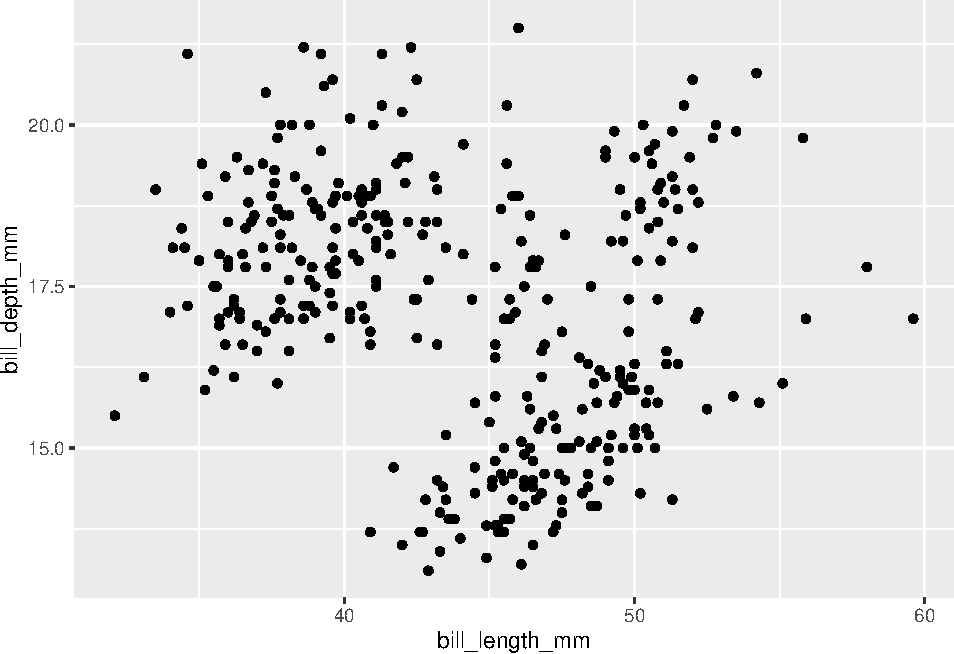
\includegraphics{thesis_files/figure-latex/unnamed-chunk-5-1.pdf}
\caption{\label{fig:unnamed-chunk-5}Penguins}
\end{figure}
\hypertarget{discussion-1}{%
\section{Discussion}\label{discussion-1}}

\hypertarget{conclusion-1}{%
\section{Conclusion}\label{conclusion-1}}

\hypertarget{process}{%
\chapter{Structure}\label{process}}

\chaptermark{process}
\begin{Shaded}
\begin{Highlighting}[]
\CommentTok{\# List of packages required for this analysis}
\NormalTok{pkg }\OtherTok{\textless{}{-}} \FunctionTok{c}\NormalTok{(}\StringTok{"dplyr"}\NormalTok{, }\StringTok{"ggplot2"}\NormalTok{, }\StringTok{"knitr"}\NormalTok{, }\StringTok{"bookdown"}\NormalTok{, }\StringTok{"devtools"}\NormalTok{)}
\FunctionTok{library}\NormalTok{(dplyr)}
\FunctionTok{library}\NormalTok{(ggplot2)}
\FunctionTok{library}\NormalTok{(kableExtra)}
\end{Highlighting}
\end{Shaded}
\hypertarget{introduction-3}{%
\section{Introduction}\label{introduction-3}}

\hypertarget{background-2}{%
\section{Background}\label{background-2}}

\hypertarget{empirical-approach-2}{%
\section{Empirical approach}\label{empirical-approach-2}}

\hypertarget{results-2}{%
\section{Results}\label{results-2}}
\begin{Shaded}
\begin{Highlighting}[]
\NormalTok{knitr}\SpecialCharTok{::}\FunctionTok{include\_graphics}\NormalTok{(}\StringTok{"\textasciitilde{}/Documents/Davis/R{-}Projects/osisn\_processes/figures/figure2.png"}\NormalTok{)}
\end{Highlighting}
\end{Shaded}
\begin{figure}
\includegraphics[width=1\linewidth]{../osisn_processes/figures/figure2} \caption{motifs}\label{fig:unnamed-chunk-6}
\end{figure}
\hypertarget{discussion-2}{%
\section{Discussion}\label{discussion-2}}

\hypertarget{conclusion-2}{%
\section{Conclusion}\label{conclusion-2}}

\hypertarget{conclusion-3}{%
\chapter*{Conclusion}\label{conclusion-3}}
\addcontentsline{toc}{chapter}{Conclusion}

If we don't want Conclusion to have a chapter number next to it, we can add the \texttt{\{-\}} attribute.

\textbf{More info}

And here's some other random info: the first paragraph after a chapter title or section head \emph{shouldn't be} indented, because indents are to tell the reader that you're starting a new paragraph. Since that's obvious after a chapter or section title, proper typesetting doesn't add an indent there.

\appendix

\hypertarget{the-first-appendix}{%
\chapter{The First Appendix}\label{the-first-appendix}}

This first appendix includes all of the R chunks of code that were hidden throughout the document (using the \texttt{include\ =\ FALSE} chunk tag) to help with readibility and/or setup.

\textbf{In the main Rmd file}

\textbf{In Chapter \ref{ref-labels}:}

\hypertarget{the-second-appendix-for-fun}{%
\chapter{The Second Appendix, for Fun}\label{the-second-appendix-for-fun}}

\hypertarget{colophon}{%
\chapter*{Colophon}\label{colophon}}
\addcontentsline{toc}{chapter}{Colophon}

This document is set in \href{https://github.com/georgd/EB-Garamond}{EB Garamond}, \href{https://github.com/adobe-fonts/source-code-pro/}{Source Code Pro} and \href{http://www.latofonts.com/lato-free-fonts/}{Lato}. The body text is set at 11pt with \(\familydefault\).

It was written in R Markdown and \(\LaTeX\), and rendered into PDF using \href{https://github.com/ryanpeek/aggiedown}{aggiedown} and \href{https://github.com/rstudio/bookdown}{bookdown}.

This document was typeset using the XeTeX typesetting system, and the University of California Thesis class. Under the hood, the elements of the document formatting source code have been taken from the \href{https://github.com/stevenpollack/ucbthesis}{Latex, Knitr, and RMarkdown templates for UC Berkeley's graduate thesis}, and \href{https://github.com/suchow/Dissertate}{Dissertate: a LaTeX dissertation template to support the production and typesetting of a PhD dissertation at Harvard, Princeton, and NYU}

The source files for this thesis, along with all the data files, have been organised into an R package, xxx, which is available at \url{https://github.com/xxx/xxx}. A hard copy of the thesis can be found in the University of XXX library.

This version of the thesis was generated on 2023-08-18 15:14:07.050859. The repository is currently at this commit:

The computational environment that was used to generate this version is as follows:
\begin{verbatim}
- Session info ---------------------------------------------------------------
 setting  value
 version  R version 4.3.0 (2023-04-21)
 os       macOS Ventura 13.4
 system   x86_64, darwin20
 ui       X11
 language (EN)
 collate  en_US.UTF-8
 ctype    en_US.UTF-8
 tz       Europe/London
 date     2023-08-18
 pandoc   3.1.1 @ /Applications/RStudio.app/Contents/Resources/app/quarto/bin/tools/ (via rmarkdown)

- Packages -------------------------------------------------------------------
 package        * version date (UTC) lib source
 aggiedown        1.0     2023-08-16 [1] Github (ryanpeek/aggiedown@ae99300)
 bookdown         0.35    2023-08-09 [1] CRAN (R 4.3.0)
 cachem           1.0.8   2023-05-01 [1] CRAN (R 4.3.0)
 callr            3.7.3   2022-11-02 [1] CRAN (R 4.3.0)
 cli              3.6.1   2023-03-23 [1] CRAN (R 4.3.0)
 colorspace       2.1-0   2023-01-23 [1] CRAN (R 4.3.0)
 crayon           1.5.2   2022-09-29 [1] CRAN (R 4.3.0)
 devtools         2.4.5   2022-10-11 [1] CRAN (R 4.3.0)
 digest           0.6.33  2023-07-07 [1] CRAN (R 4.3.0)
 dplyr          * 1.1.2   2023-04-20 [1] CRAN (R 4.3.0)
 ellipsis         0.3.2   2021-04-29 [1] CRAN (R 4.3.0)
 evaluate         0.21    2023-05-05 [1] CRAN (R 4.3.0)
 fansi            1.0.4   2023-01-22 [1] CRAN (R 4.3.0)
 farver           2.1.1   2022-07-06 [1] CRAN (R 4.3.0)
 fastmap          1.1.1   2023-02-24 [1] CRAN (R 4.3.0)
 fs               1.6.3   2023-07-20 [1] CRAN (R 4.3.0)
 generics         0.1.3   2022-07-05 [1] CRAN (R 4.3.0)
 ggplot2        * 3.4.3   2023-08-14 [1] CRAN (R 4.3.0)
 glue             1.6.2   2022-02-24 [1] CRAN (R 4.3.0)
 gtable           0.3.3   2023-03-21 [1] CRAN (R 4.3.0)
 highr            0.10    2022-12-22 [1] CRAN (R 4.3.0)
 htmltools        0.5.6   2023-08-10 [1] CRAN (R 4.3.0)
 htmlwidgets      1.6.2   2023-03-17 [1] CRAN (R 4.3.0)
 httpuv           1.6.11  2023-05-11 [1] CRAN (R 4.3.0)
 httr             1.4.7   2023-08-15 [1] CRAN (R 4.3.0)
 kableExtra     * 1.3.4   2021-02-20 [1] CRAN (R 4.3.0)
 knitr          * 1.43    2023-05-25 [1] CRAN (R 4.3.0)
 labeling         0.4.2   2020-10-20 [1] CRAN (R 4.3.0)
 later            1.3.1   2023-05-02 [1] CRAN (R 4.3.0)
 lifecycle        1.0.3   2022-10-07 [1] CRAN (R 4.3.0)
 magrittr         2.0.3   2022-03-30 [1] CRAN (R 4.3.0)
 memoise          2.0.1   2021-11-26 [1] CRAN (R 4.3.0)
 mime             0.12    2021-09-28 [1] CRAN (R 4.3.0)
 miniUI           0.1.1.1 2018-05-18 [1] CRAN (R 4.3.0)
 munsell          0.5.0   2018-06-12 [1] CRAN (R 4.3.0)
 palmerpenguins * 0.1.1   2022-08-15 [1] CRAN (R 4.3.0)
 pillar           1.9.0   2023-03-22 [1] CRAN (R 4.3.0)
 pkgbuild         1.4.2   2023-06-26 [1] CRAN (R 4.3.0)
 pkgconfig        2.0.3   2019-09-22 [1] CRAN (R 4.3.0)
 pkgload          1.3.2.1 2023-07-08 [1] CRAN (R 4.3.0)
 prettyunits      1.1.1   2020-01-24 [1] CRAN (R 4.3.0)
 processx         3.8.2   2023-06-30 [1] CRAN (R 4.3.0)
 profvis          0.3.8   2023-05-02 [1] CRAN (R 4.3.0)
 promises         1.2.1   2023-08-10 [1] CRAN (R 4.3.0)
 ps               1.7.5   2023-04-18 [1] CRAN (R 4.3.0)
 purrr            1.0.2   2023-08-10 [1] CRAN (R 4.3.0)
 R6               2.5.1   2021-08-19 [1] CRAN (R 4.3.0)
 Rcpp             1.0.11  2023-07-06 [1] CRAN (R 4.3.0)
 remotes          2.4.2.1 2023-07-18 [1] CRAN (R 4.3.0)
 rlang            1.1.1   2023-04-28 [1] CRAN (R 4.3.0)
 rmarkdown        2.24    2023-08-14 [1] CRAN (R 4.3.0)
 rstudioapi       0.15.0  2023-07-07 [1] CRAN (R 4.3.0)
 rvest            1.0.3   2022-08-19 [1] CRAN (R 4.3.0)
 scales           1.2.1   2022-08-20 [1] CRAN (R 4.3.0)
 sessioninfo      1.2.2   2021-12-06 [1] CRAN (R 4.3.0)
 shiny            1.7.5   2023-08-12 [1] CRAN (R 4.3.0)
 stringi          1.7.12  2023-01-11 [1] CRAN (R 4.3.0)
 stringr          1.5.0   2022-12-02 [1] CRAN (R 4.3.0)
 svglite          2.1.1   2023-01-10 [1] CRAN (R 4.3.0)
 systemfonts      1.0.4   2022-02-11 [1] CRAN (R 4.3.0)
 tibble           3.2.1   2023-03-20 [1] CRAN (R 4.3.0)
 tidyselect       1.2.0   2022-10-10 [1] CRAN (R 4.3.0)
 urlchecker       1.0.1   2021-11-30 [1] CRAN (R 4.3.0)
 usethis          2.2.2   2023-07-06 [1] CRAN (R 4.3.0)
 utf8             1.2.3   2023-01-31 [1] CRAN (R 4.3.0)
 vctrs            0.6.3   2023-06-14 [1] CRAN (R 4.3.0)
 viridisLite      0.4.2   2023-05-02 [1] CRAN (R 4.3.0)
 webshot          0.5.4   2022-09-26 [1] CRAN (R 4.3.0)
 withr            2.5.0   2022-03-03 [1] CRAN (R 4.3.0)
 xfun             0.40    2023-08-09 [1] CRAN (R 4.3.0)
 xml2             1.3.5   2023-07-06 [1] CRAN (R 4.3.0)
 xtable           1.8-4   2019-04-21 [1] CRAN (R 4.3.0)
 yaml             2.3.7   2023-01-23 [1] CRAN (R 4.3.0)

 [1] /Library/Frameworks/R.framework/Versions/4.3-x86_64/Resources/library

------------------------------------------------------------------------------
\end{verbatim}
\hypertarget{references}{%
\chapter*{References}\label{references}}
\addcontentsline{toc}{chapter}{References}

Placeholder

\end{ucmainmatter}
\end{document}

%---Set Headers and Footers ------------------------------------------------------
\pagestyle{fancy}
\renewcommand{\chaptermark}[1]{\markboth{{\sf #1 \hspace*{\fill} Chapter~\thechapter}}{} }
\renewcommand{\sectionmark}[1]{\markright{ {\sf Section~\thesection \hspace*{\fill} #1 }}}
\fancyhf{}

\makeatletter \if@twoside \fancyhead[LO]{\small \rightmark} \fancyhead[RE]{\small\leftmark} \else \fancyhead[LO]{\small\leftmark}
\fancyhead[RE]{\small\rightmark} \fi

\def\cleardoublepage{\clearpage\if@openright \ifodd\c@page\else
  \hbox{}
  \vspace*{\fill}
  \begin{center}
    This page intentionally left blank
  \end{center}
  \vspace{\fill}
  \thispagestyle{plain}
  \newpage
  \fi \fi}
  
\makeatother
\fancyfoot[c]{\textrm{\textup{\thepage}}} % page number
\fancyfoot[C]{\thepage}
\renewcommand{\headrulewidth}{0.4pt}

\fancypagestyle{plain} { \fancyhf{} \fancyfoot[C]{\thepage}
\renewcommand{\headrulewidth}{0pt}
\renewcommand{\footrulewidth}{0pt}}
